% Outline Project Specification Report

%The document is a report
\documentclass[12pt,a4paper]{article}

%define horizontal rule
\newcommand{\HRule}{\rule{\linewidth}{0.5mm}}

\usepackage{fullpage}

%use the listings package
\usepackage{listings}
%use the English language
\usepackage[english]{babel}
%use graphics
\usepackage{graphicx}
%use wrap figures
\usepackage{wrapfig}
%geometry stuffs
\usepackage{lscape}
%use natbib bibliography package
%\usepackage[numbers]{natbib}
%use harvard bibliography package
%\usepackage{harvard}	
%use captions
\usepackage{caption}
%use multi-row tables
\usepackage{multirow}
\usepackage{url}
\usepackage{subcaption}


\usepackage[nottoc,numbib]{tocbibind}

\begin{document}

%use harvard citations
%\citationstyle{agsm}

%include the title page
\newcommand{\Revision}{678f948}

\begin{titlepage}
 
\begin{center}

% Upper part of the page

\includegraphics[width=0.20\textwidth]{../cover_logo.png}\\[1cm]


\textsc{\LARGE Aberystwyth University}\\[0.5cm]
\textsc{\LARGE Final Report}\\[0.5cm]



 
% Title
\HRule \\[0.4cm]
{ \huge \bfseries Partridge: An Intelligent Literature Analysis and
Recommendation Suite.}\\[0.4cm]

\HRule \\[1.5cm]

 % Author and student ID
\begin{minipage}{0.4\textwidth}
\begin{flushleft} \large
\emph{Author:}\\
\textsc{James Ravenscroft}\\
jrr9@aber.ac.uk\\
090407039\\
\end{flushleft}
\end{minipage}
\begin{minipage}{0.4\textwidth}
\begin{flushright} \large
\emph{Supervisors} \\
Amanda Clare (afc)\\
Maria Liakata (mal)

\end{flushright}
\end{minipage}


\vfill

\textsc{Submitted in partial fulfilment of requirements for a Batchelor of
Science Degree at Aberystwyth University}



\vfill
 
% Bottom of the page
\textsc{\large Word Count: 0}\\
\textsc{\large Status: Draft}\\
\textsc{\large Revision: \Revision{} }\\
{\large \today}
 
\end{center}

\frontmatter
 
\end{titlepage}



%some definitions for paragraph layout stuff
\setlength{\parindent}{0pt}
\setlength{\parskip}{1.5ex plus 0.5ex minus 0.2ex}

\tableofcontents

\pagebreak

\section{Project Summary}

Partridge is a web-based tool designed to assist in information processing and knowledge
acquisition within the domain of scientific research.

Since the advent of the 'Digital Age' and the ability of computers to copy and
reproduce information for a negligible cost, the amount of information
available to researchers has been increasing drastically.  B-C Bj\"{o}rk (2009)
estimates that approximately 1.4 Million papers were published in the year 2006
alone\cite{bjork2009}. Moreover, the growing popularity of Open Access
publishing (making papers available for free online\cite{Suber2012}) across
most scientific disciplines\cite{bjork2009}\cite{harnad2004comparing} is
providing researchers with an even larger volume of information to be
processed. As available information increases, relevant material becomes
progressively more difficult to find and the need for an automated information
retrieval tool more apparent. The problem is even more vital for General
Practitioners. Goldacre (2008:97) points out that ``there have been an
estimated 15 million medical academic articles published so far, and 5000
journals published every month... picking out what's relevant is a garganutan
task."\cite{goldacre2008bad} 

Partridge aims to autonomously process as many scientific papers as possible to
facilitate researchers who would otherwise be required to manually read each
paper themselves. This should reduce the amount of information that the reader
is required to process themselves, thereby speeding up the research process.
Partridge will achieve this through the use of several existing techniques in
Natural Language Processing which are discussed below.

From the point of view of it's users, Partridge will assist researchers in two
ways. The system will provide filtering of papers based upon their
specific domain (i.e. is the paper primarily concerned with methodology within
an experiment in chemistry or is it about ethics in psychological studies?) and
their result, whether the paper yielded positive, negative or inconclusive
evidence for a hypothesis. Depending upon the time constraints of the
project, it is hoped that Partridge will also offer a user 'profiling' system
that provides recommendations for researchers based on their reading history.
This feature should help users find relevant papers more quickly or find
research that they may have otherwise overlooked.

There are already several tools that help researchers manage the vast library
of journals available on the internet. Search engines such as Google
({\url{http://www.google.com/}}), and social citation management tools such as
CiteULike ({\url{http://www.citeulike.org}}), do offer some assistance in
tracking down relevant information. However, these tools are often too general
or rely upon the user knowing exactly what keywords to use before carrying out
the search. These drawbacks are further discussed in Section
\ref{sec:prior_art} below.

To overcome the drawbacks of these existing systems, Partridge will make use of
several cutting edge Artificial Intelligence (AI) techniques in order to analyse and
process the papers in a more in depth way. AI is a very complex and field and
implementing the above features will be incredibly challenging. To help with
this, Partridge will build upon the system implemented by Liakata et al. for
classifying papers on a sentence-by-sentence basis\cite{citeulike:10444769} and
make use of Natural Language Toolkit for Python
\cite{bird2009natural} 

\section{Current Progress}

\subsection{Literature Review}

In science fiction literature and films, Artificial Intelligence (AI) and the
ability of machines to automatically process and understand human language is
almost always taken for granted. The current state of AI is a long way behind these
fantastic visions. Dale(2000) comments that ``Even the most ardent exponent of
artificial intelligence research would have to admit that the likes of HAL in
Kubrick's 2001: A Space Odyssey remain firmly in the realms of science
fiction\cite{dale2000handbook}".

Despite lacking behind the imagination of authors and script writers, over the last 60 years there
has been a huge amount of progress in AI techniques. The phrase `Artificial
Intelligence' was coined in 1956\cite{russell2010artificial} and can be used as
an umbrella term, describing many subfields from ``learning and perception
to... diagnosing diseases\emph{(Ibid)}."

Turing(1950) proposed a test for determining whether a machine could be
considered intelligent or not\cite{turing1950computing}. Turing's test is based
upon whether a computer can communicate in a natural language proficiently
enough to deceive a human into thinking that the machine is also human. A
machine able to pass such a test would need to possess the ability to represent
and learn from knowledge, to be able to reason about what it knows and to be
able to process natural language\cite{russell2010artificial}. Partridge will
also need to be able to process natural language and learn from any
observations it makes. It is reasonable to consider Partridge's backend system
to be an Artificial Intelligence problem. Primarily, Patridge can be considered
a Natural Language Processing problem.


\subsubsection{Natural Language Processing} 

Natural Language Processing (NLP) is still a relatively unexplored discipline
and as such is a very active area of research and development within the AI
community\cite{liddy2001natural}. NLP enables the automated extraction of
meaningful information from texts written in human languages such as English or
French. NLP has already been applied to many text classification and data
extraction problems. Studies have been carried out in the detection of emotions
in suicide notes\cite{citeulike:11077287}, the classification of a web page's
genre on the World Wide Web\cite{citeulike:11288938} and emotional polarity
(determining the positive or negative implications of) of a phrase or
sentence\cite{Wilson05Polarity}. Liddy(2001) defines Natural Language
Processing as:

\begin{quotation} 
A theoretically motivated range of computational techniques for analyzing and
representing naturally occurring texts at one or more levels of linguistic
analysis for the purpose of achieving human-like language processing for a
range of tasks or applications \it{(Ibid)}.  
\end{quotation}

In the case of Partridge, scientific papers, constituting the naturally occuring
texts, are processed at sentence-by-sentence and word-by-word levels of
linguistics and represented in the form of Extended Markup Language (XML)
documents, a format that is both human and machine readable. This information
is then used for the purpose of classifying and searching papers in a
human-like way. 

It is therefore necessary to define what a 'human-like way' of processing
scientific papers.  Krug (2005), suggests that when browsing the internet,
humans find it much easier to locate specific information within a labelled and
logically structured document than one that is provided as a single text
entity\cite{Krug:2005:DMM:1051204}. In order to help humans to find relevant
research papers, Partridge will represent all papers in its repository in a
logical hierarchical structure. This will facilitate better information
retrieval for keyword searches and enable more advanced NLP techniques.
Partridge's document storage format should therefore be standardised to provide
a uniform way of processing each document. 

\subsubsection{CISP, CoreSC and SAPIENTA}

Soldatova and Liakata(2007) proposed a methodology for storing the Core
Information about Scientific Papers (CISP) as a way to formally represent
scientific concepts that should be present in the articles in a logical
ontology\cite{soldatova2007ontology}. They then proceed to define a schema for
their CISP ontology that defines the Core Scientific Concepts (CoreSC) as part
of the XML document itself\cite{liakata2008guidelines}. 

It is proposed that Partridge uses the CoreSC schema for document storage
to provide a standard way to access and process the papers and thus
eliminate dealing with multiple documents during its learning phase. 
Using CoreSC also offers the advantage of making Partridge compatible
with the ART corpus. This is a set of physical chemistry and biochemistry
research papers that have been pre-processed and already annotated using CISP
concepts\cite{liakataART}. This would provide Partridge with a set of papers
that could be used as a training set for classification tasks and could be used
for information retrieval tests from early on in the project.

Liakata et al. (2012) describe a system for automatically processing and
categorising sentences in a research paper according to their respective CoreSC
element\cite{citeulike:10444769}. SAPIENTA
(\url{http://www.sapientaproject.com}) was trained using the ART corpus and can
achieve promising accuracies when categorising sentences (\emph{Ibid}). With
the authors' permissions, Partridge will make use of SAPIENTA when introducing
new papers into its repository. It is hoped that preclassifying papers with
SAPIENTA will make the development of Partridge more manageable within the
timeframe available and will also allow more effort to be put into other
classification problems rather than re-implementing a SAPIENTA clone. Any
modifications that have to be made to SAPIENTA to integrate it into Partridge
will be submitted back to the original authors to assist them in their research.

After pre-processing by SAPIENTA is complete, Partridge will need to do some
classification work of its own to determine the area of study (i.e. Physics,
Chemistry, Biology), type of paper (Literature review, Case Study, Experiment)
and the polarity of the result (positive, negative, inconclusive). These tasks
involve implementing existing AI techniques and applying them specifically to
the task of text classification. To avoid the time consuming task of
re-implementing these methods, it was decided that a library should be used
instead. Different NLP libraries and their properies are discussed below in
Section \ref{sec:libschoice}.


\subsection{Related Works}
\label{sec:prior_art}

\subsubsection{Search Engines} 

There are already many existing systems for finding and filtering information
on the World Wide Web. Search engines are very useful for information retrieval
in the very large and generalised search domain of the Internet. Most people
have heard of Google (\url{http://wwww.google.com}), Yahoo
(\url{http://www.yahoo.co.uk}), Bing (\url{http://www.bing.com}) and Ask
(\url{http://www.ask.com}). There are many more similar systems available for
free general use across the internet.  They all present very similar user
interfaces (as shown in Figure \ref{fig:search_interfaces}) in which users are
asked to supply keywords that might be linked to relevant documents and the
search engine returns a list of Uniform Resource Locators (URLs) that they
consider to match the user's query.


\begin{figure}[!ht]
        \centering
        \begin{subfigure}[b]{0.50\textwidth}
                \centering
                
\includegraphics[width=\textwidth]{images/ask_front.png}
                \caption{Ask.com}
                \label{fig:ask_interface}
        \end{subfigure}%
        \begin{subfigure}[b]{0.50\textwidth}
                \centering
                
\includegraphics[width=\textwidth]{images/bing_front.png}
                \caption{Bing.com}
                \label{fig:bing_interface}
        \end{subfigure}\\
        \begin{subfigure}[b]{0.50\textwidth}
                \centering
                
\includegraphics[width=\textwidth]{images/google_front.png}
                \caption{Google.com}
                \label{fig:google_interface}
        \end{subfigure}%
        \begin{subfigure}[b]{0.50\textwidth}
                \centering
                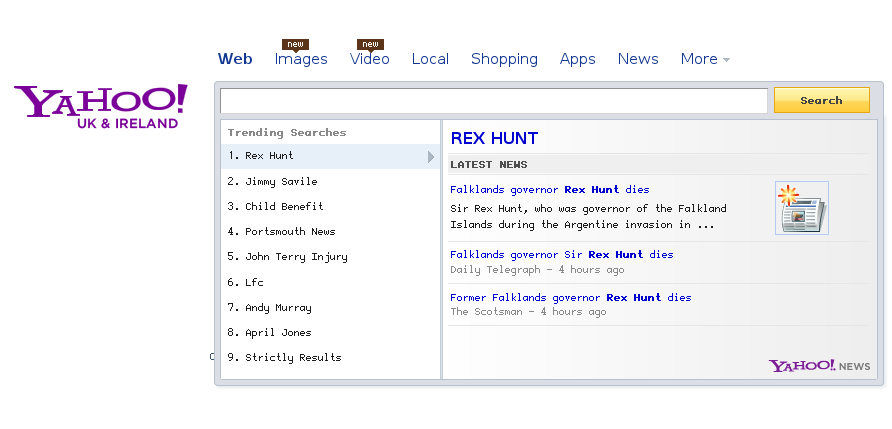
\includegraphics[width=\textwidth]{images/yahoo_front.png}
                \caption{Yahoo.com}
                \label{fig:yahoo_interface}
        \end{subfigure}%
        \caption{4 popular search engine interfaces}\label{fig:animals}
        \label{fig:search_interfaces}
\end{figure}


Search engines are helpful in locating pages and websites within the World Wide
Web. Unfortunately, the problem space they deal with is usually too big for
them to find scientific papers and journals given a set of keywords. Internet
search engines index a huge proportion of irrelevant information compared to
useful information\cite{Berghel1997}, and as a result, even relatively specific
queries such as ``effects of gravity on rockets" yield millions of results (as
shown in Figure \ref{fig:rocket_results}). 

\begin{figure}[!ht]
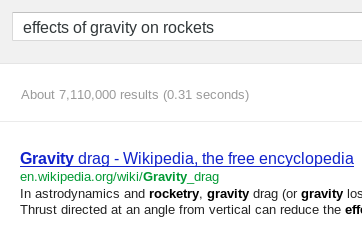
\includegraphics[width=0.80\textwidth]{images/space_rocket_query.png}
\caption{{Google showing over 7M results for ``effects of gravity on rockets"}}
\label{fig:rocket_results}
\end{figure}

Partridge offers an advantage over these mechanisms as it will specifically
index research papers rather than attempting to index the whole Internet.
This means that there should be a higher proportion of useful information as
output compared to the output of an Internet Search Engine.

\subsubsection{Scientific Paper Search Engines}
There are also a number of search and indexing systems that specifically look
for scientific papers as opposed to web pages. One of the most publicised and
well known paper search systems is Google Scholar
(\url{http://scholar.google.com}).  As can be seen in Figure
\ref{fig:scholar_basic}, This is an adaptation of Google's general search
engine (discussed above) to specifically index and search scientific papers.
Google also offers advanced query options specific to Scholar that allow
searching by author, year and for words that occur only in the document title
as shown in figure \ref{fig:scholar_advanced}. Whilst this does deal with the
problem of `information overload' and provides even more fine control over the
information returned from searches,  the user is still required to have a very
good idea of what they are looking for in terms of keywords and/or specific
authors. It is possible that a user would not know what they are looking for
until they've seen it. Even if the user has a set of keywords to search for,
they can only search the title of the paper or the content as a whole. This
means that users who want to find a particular phrase within a CoreSC part of
the paper (e.g. only look for this phrase in the `Result' section of the
paper) are unable to get results at their desired level of detail.

\begin{figure}[!hbt]
        \centering
        \begin{subfigure}[b]{0.50\textwidth}
                \centering
                
\includegraphics[width=\textwidth]{images/googlescholar_front.png}
                \caption{Google Scholar's General front page}
                \label{fig:scholar_basic}
        \end{subfigure}%
        \begin{subfigure}[b]{0.50\textwidth}
                \centering
                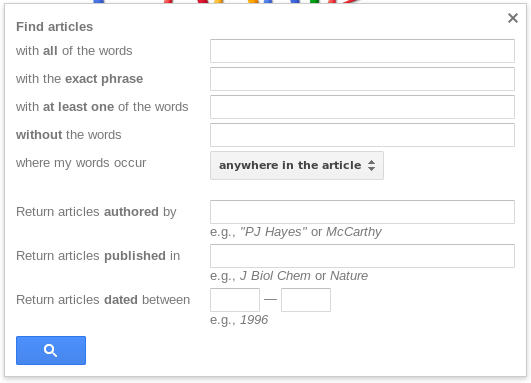
\includegraphics[width=\textwidth]{images/googlescholar_advanced.png}
                \caption{Advanced search features}
                \label{fig:scholar_advanced}
        \end{subfigure}

        \caption{Google Scholar's user interface}
        \label{fig:scholar_interface}
\end{figure}

Partridge will provide the option to filter papers by subject and it is hoped
that the system will also provide user-specific recommendations by profiling
them through their reading history. This will make it easier for users to find
relevant papers without knowing exactly which keywords they need to search for.
Partridge will also offer facilitate searching for keywords within a specific
CoreSC section by making use of Liakata et al's SAPIENTA project for
classifying each sentence of paper as it is added to the repository.

\subsubsection{Social Citation and Recommendation Engines}
Social citation and recommendation engines also provide a partial solution to
the `information overload' problem.  Services like Goodreads
(\url{http://www.goodreads.com/}) and CiteUlike
(\url{http://www.citeulike.org/}) allow you to register your interest in
specific authors and subjects. This allows the sites to build up a profile of
the sorts of materials that you might be interested in and provide lists of
recommendations as in Figure \ref{social_indexes}.

\begin{figure}[!hbt]
        \centering
        \begin{subfigure}[b]{0.50\textwidth}
                \centering
                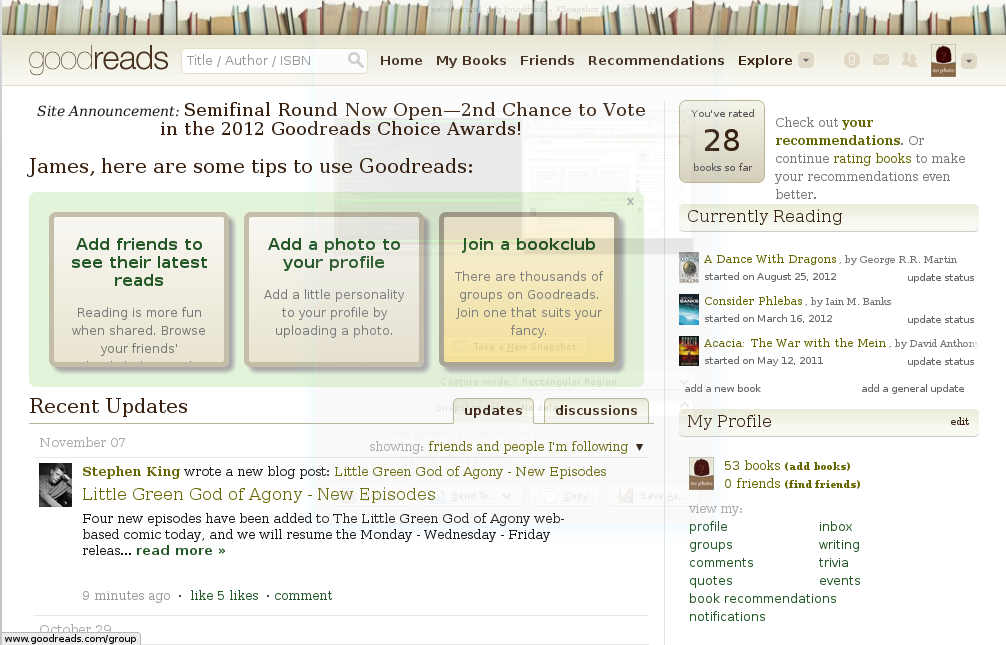
\includegraphics[width=\textwidth]{images/goodreads_index.png}
                \caption{Goodreads user profile page}
                \label{fig:goodreads_index}
        \end{subfigure}%
        \begin{subfigure}[b]{0.50\textwidth}
                \centering
                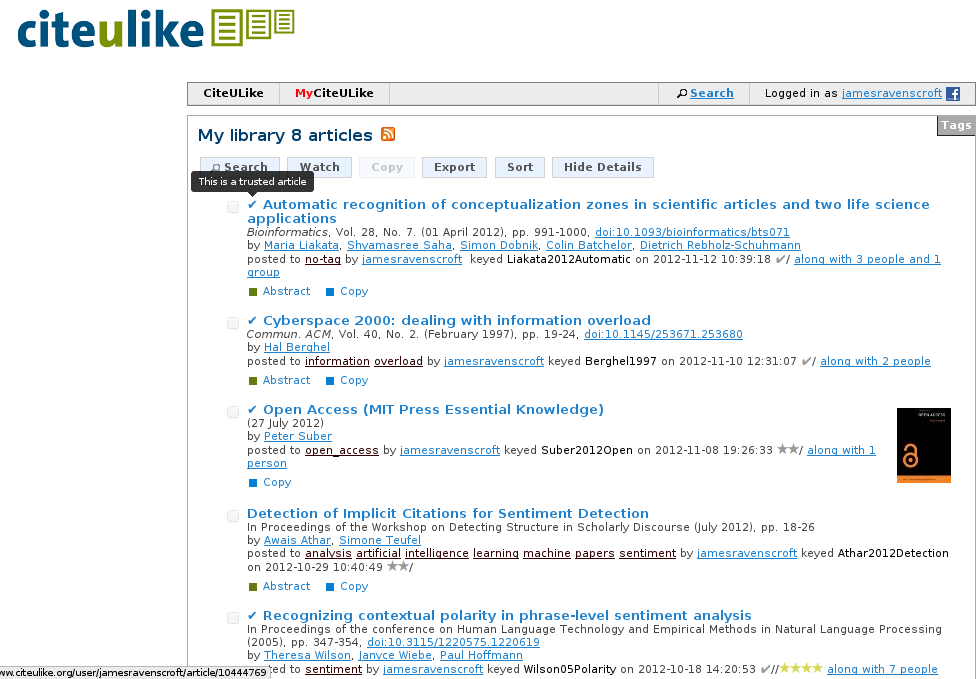
\includegraphics[width=\textwidth]{images/citeulike_index.png}
                \caption{a CiteULike user profile page}
                \label{fig:citeulike_index}
        \end{subfigure}

        \caption{Goodreads and citeulike social recommendation systems}
        \label{fig:social_indexes}
\end{figure}

These systems have the ability to make recommendations to the user without
requiring specific keywords or search terms. They do this by learning the
user's profile and taking into account the preferences of their 'friends' and
their browsing history. However, the above-named systems do not take into
account the content of the paper or book. They only deal with metadata as can
be seen in Figure \ref{fig:social_searches}. This means that important
discriminatory information that could be contained within the actual document
content is overlooked completely. Partridge will analyse documents on a
sentence-by-sentence and possibly word-by-word basis, thereby taking account of
any embedded information that could be missed by these social metadata systems.

\begin{figure}[!hbt]
        \centering
        \begin{subfigure}[b]{0.50\textwidth}
                \centering
                
\includegraphics[width=\textwidth]{images/goodreads_search.png}
                \caption{Goodreads advanced search page}
                \label{fig:goodreads_search}
        \end{subfigure}%
        \begin{subfigure}[b]{0.50\textwidth}
                \centering
                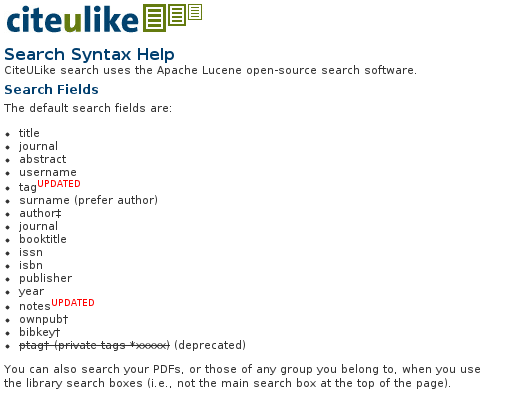
\includegraphics[width=\textwidth]{images/citeulike_search.png}
                \caption{CiteULike advanced search options}
                \label{fig:citeulike_search}
        \end{subfigure}

        \caption{Goodreads and citeulike search only deal with metadata.}
        \label{fig:social_searches}
\end{figure}


\subsection{Methodology}

The language that Partridge will be written in is one of the most fundamental
and important choices to be made. The language choice effects not only the end
performance of the application, but the speed at which the project is developed
and the portability of the end code \cite{britton2008}. To avoid a learning
overhead, it was decided that the programming language should be one that the
author is familiar with. This reduced the choice of language down to C, Java
and Python. 

The C programming language was invented by Kernighan and Ritchie and
published in 1978\cite{ritchie1978c}. The language is small and
optimised\cite{prinz2002c} and therefore compiled C programs tend to run
extremely fast. Unfortunately, C is designed to be general and lack restriction
\cite{ricthie1978c} which is often an advantage for programmers who favour
optimised code over excessive error checking. However, this means that
debugging C programms can be quite long winded and challenging. Since the NLP
aspects of Partridge present an amibitious challenge in themselves, having to
debug applications without help from a managed programming environment is not
desirable. 

The Java programming language on the other hand, does provide memory management
and error checking\cite{Coffey2008} at the cost of program performance. Java is
a pseudo-compiled language that is translated into bytecode then interpreted at
runtime by a Virtual Machine(VM) on the client computer. Gosling (2000)
describes java as a ``general-purpose...  programming language [that allows]
developers to write a program once and then be able to run it everywhere on the
internet\cite{gosling2000java}." Java provides a stable programming environment
and error checking, both of which would be advantageous in the development of
Partridge. Java's syntax is very verbose and a lot of `boiler-plate' code must
be written before a program can be executed.  Therefore Java is not suitable as
a rapid prototyping language. Since Partridge's development requires a steep
learning curve for the author, a language that allows quick prototyping with
minimal programming.

Python is a programming language with a famously shallow learning curve,
readable syntax and dynamic inspection that facilitates rapid prototyping
\cite{bird2009natural}. The language was invented by Guido Van Rossum as a
multi-use, flexible, interpreted scripting language, extensible via compiled C
modules\cite{An93pythonfor}. Developing Partridge in python
would provide a flexible prototyping environment and readable syntax allowing
for investigative work to be carried out quickly and efficiently with minimal
overheads for writing boiler-plate code and debugging. The ability to extend
the language using native code would give Partridge an even greater advantage.
Since NLP techniques can be quite processor intensive and Python is an
interpreted language, and in its very nature, slower than a compiled language,
inefficient sections of Python code could be re-written as C extensions and
compiled into the application. For these reasons, Python was selected as the
preferred programming language for Partridge development.

\subsubsection{Web Presentation Frameworks} 

Partridge's web frontend will be used by researchers to wish to query the
system for information on scientific papers. As it is a web tool, Partridge
will be presented as a set of HTML web pages. 

It is possible to use a separate software stack Such as Apache web server
(\url{http://httpd.apache.org/}) and PHP (\url{http://www.php.net}) as a web
presentation layer. However, this would involve adding more software to the
project and building an interface between the PHP scripts and Partridge's
python backend. To prevent unnecessary complication, this approach will be
avoided and instead, a Python web toolkit will be used and integrated directly
with the backend.

Django (\url{http://www.djangoproject.com/}) is a Python web framework with
integrated database management and templating capabilities \cite{django2012}.
The framework provides automatic management of all aspects of your
application's data storage systems unless explicitely disabled. The framework
also uses a fairly stricty Model-View-Controller pattern and this is enforced
in the structure of the application code. These features may be useful in a
general web application such as a news site. Partridge requires a much more
complex internal structure to take into account the machine learning and NLP
aspects of the system. Having to `shoehorn' Partridge into a specific structure
to make it compatible with Django adds extra overhead to the project and is not
desirable.

Flask (\url{http://flask.pocoo.org}) is a python `microframework' for web
development. Ronacher (2012) writes that ``Flask aims to keep the core simple
but extensible...[and] won't make any decisions for you\cite{flask2012}." It
uses a simple templating system that can optionally be swapped out for an
equivalent system and does not impose any limitations or requirements on the
layout of the program or the type of database that is used. Flask integrates
very simply into existing software using Python annotations\emph{(Ibid)}. This approach
means that the framework could be adapted to Partridge very quickly, rather
than requiring Partridge to be adapted to the framework. Therefore, Flask has
been chosen as the preferred web framework for use in the project.

\subsubsection{Natural Language Libraries} \label{sec:libschoice}.  There are
several existing libraries to facilitate Natural Language Processing.  Many are
written for Java \cite{mallet2002}\cite{cunningham2011text} and are very
complex or not well documented. The Natural Language Toolkit (NLTK) is a simple
and intuitive library written for Python. Bird(2009) states that NLTK was
designed ``to provide an intuitive framework along with substantial building
blocks, giving users a practical knowledge of NLP\cite{bird2009natural}". The
project is relatively mature in comparison to the above named Java libraries.
There is also a free book that accompanies the project available at
\url{http://nltk.org/book/} which provides a huge amount of information on how
to implement many popular NLP techniques using the library. For this reason
NLTK was chosen as the primary accompanying library for the project.

\subsection{Prototyping/Current Work}

\subsubsection{PDF Conversion}
Most scientific papers available on the internet are formatted as PDF
documents. However, Partridge uses and stores documents that use the CoreSC
schema by Soldatova and Liakata\cite{liakata2008guidelines}. Therefore some
spike work was carried out to determine the feasibility of converting papers
published as PDF documents into XML documents. Townsendi et al(2009) liken converting
PDF to XML to ``converting hamburgers into cows," they go on to explain that
PDF documents do not contain any semantic data and documents lose much of their
explicit structure when they are formatted in this way \cite{Townsend2009}.
Therefore, to convert PDF documents into an NLP-friendly format, some
heuristics must be used to detect the document's structure\cite{pdfminer}. 

A prototype script was written using a Python PDF extraction library called
PDFMiner (\url{http://www.unixuser.org/~euske/python/pdfminer/index.html}).
This toolkit already contains some heuristics about how to extract text from
PDF documents in a sane way\cite{pdfminer}. The script then used the NLTK
library to split the text into sentences and save the document in a CoreSC
compatible format for processing by SAPIENTA. 

The script had limited success due to the high variation of formatting within
scientific papers. It was suggested that PDFX (\url{http://pdfx.cs.man.ac.uk/})
a free service hosted by the university of manchester, could be used instead of
PDFMiner. PDFX's main advantage is that it uses a machine learning system to
guess PDF document structures more accurately than through the use of simple
Heuristics. With an adapted backend that sends PDFs for analysis using PDFX and
then splits the results using NLTK, the conversion script now has a much higher
success rate and will be used as a preprocessor for adding PDF  documents to
Partridge.

\subsubsection{Interface Design}

To help in visualising how the final web frontend will appear, some diagrams of
the user interface have been drawn. You can see these diagrams in Appendix
\ref{sec:ui_designs}. 

\subsubsection{System Processes}

To visualise how some of the system processes will work and how they should be
programmed, some flow diagrams have been produced and attached in Appendix
\ref{sec:system_diagrams}

\section{Planning}

\subsection{Development Methodology}

\subsubsection{Existing Methodologies}
Selecting a suitable development methodology for building Partridge is another
very important choice for the project.

Under the traditional `Waterfall' Software Development model, Requirements
Gathering, Analysis, Program Design, Coding, Testing and Operations were all
defined as formal phases in the development cycle. There is little flexibility
other than moving back up the waterfall to rectify mistakes after
testing\cite{Royce:1987:MDL:41765.41801}. This model was very focused on
paperwork and bureaucracy, trying to maintain a paper trail and manage risk
through accountability \emph{(Ibed)}. This approach to software development is
very heavyweight and slow and often produced software that did not match the
users' needs as a result \cite{Boehm1988}.

As an alternative to the heavyweight Waterfall approach, Beck et al came up
with the principle of the Agile Manifesto, favouring a lightweight, responsive
development model over the heavyweight slow waterfall
system\cite{beck2001agile}. Many of Beck's ideas focus around working in a team
of developers and prioriting communication between team members \emph{(Ibid)}.
This is most prominent in the Extreme Programming (XP) method of software
development. Since Partridge is an individual project, XP is not really
applicable. However, some concepts like rapid prototyping/spike work and
iterative release cycles will be used as part of the Partridge development
methodology.

\subsubsection{ Partridge's Development Methodology}

Partridge is an individual project but does involve discussions with
supervisors. The customers have been identified as the end-users of the system.
Therefore, a customised methodology has been adopted. Firstly, all design and
planning documentation have been written up and placed on a wiki which is
accessible and modifiable by the author and both supervisors. This creates a
paper trail for all tasks and also allows collaboration between involved
parties through the Internet. A full printout of the wiki is available in
Appendix \ref{sec:wiki}. 

Weekly meetings are held with both supervisors. The notes from the preceeding
week are analysed and each task discussed in depth. New tasks are then noted
down along with any observations that should be documented. These new notes are
uploaded to the wiki the following day or earlier. Each party present at the
meeting adds their own observations to the notes page. This page is then
reviewed at the next meeting. As seen in Appendix \ref{sec:wiki}, this practice
has already been running for several weeks and has so far proven to be highly
effective.

Partridge will adopt an Agile approach to release cycles, producing a working
software package at iterations of one month.  Each iteration, the software will
include more of the desired functionality discussed above and in the wiki.
GitHub's issue manager program is being used to track tasks and bugfixes and
plan which tasks will be carried out in which iteration. Tasks that are created
in a full iteration (where no development time is left) will be added to a
backlog and integrated in the next iteration with enough development time to
contain it. Tasks are also assigned a priority, higher priority issues being
tackled before low priority ones.

Partridge's testing strategy consists of multiple unit tests that are run at
integration of new code into the codebase. As soon as the first release is
built, Partridge will be made available for use by the public and users
encouraged to test the system and submit any bugs via the GitHub issue manager.
It is hoped that colleagues at Aberystwyth University and Dr. Liakata's
colleages at the EBI will try to use the system one it becomes available.

\subsubsection{ Work Timeline }

The tasks involved in Partridge have been carefully calculated and prioritised.
They were then added to the GitHub issue management system and a report
generated listing them in the order that they are expected to be
accomplished. This report can be seen in Appendix \ref{sec:timeline}. 


\subsubsection{ Mid-Project Demonstration Plan}

The mid-project demonstration is scheduled for after iteration two of the
Partridge project. If everything runs to schedule, then at this point it will
be possible to demonstrate keyword search within the project's database and
filter based upon the polarity of the paper's results. For redundancy purposes,
Partridge will be configured to run as a server on multiple computers. Both
this and the final project demonstration will require a room with Internet
access. However, should this be unavailable, then Partridge could be run
locally on the author's laptop.

\subsubsection{ Final Project Demonstration Plan}

The final demonstration of Partridge will be fairly similar to the Mid-Project
demonstration. However, it should include all of the planned classifiers and if
there is extra time on the project, the profiling/recommendation engine will
also be demonstrated. This demonstration will use the same redundancy
precautions as the Mid-project demonstration above, and will also need a room
with the internet if available.

\appendix
\section{User Interface Designs}
\label{sec:ui_designs}

\section{System Process Diagrams}
\label{sec:system_diagrams}


\section{Project Timeline}
\label{sec:timeline}

\section{Project Wiki}
\label{sec:wiki}


\bibliographystyle{IEEEannot}
\bibliography{report}

\end{document}
